\chapter{Introdução}
\label{cap:p1}
Este primeiro capítulo tem como objetivo apresentar uma breve introdução ao exercício a realizar. Sendo assim, é necessário perceber os motivos que levaram à resolução do exercício assim como os objetivos pretendidos.

A extensão à programação em lógica surge da necessidade de abandonar conceitos restritos obrigatoriamente associados à programação em lógica abordada no primeiro trabalho prático.
A extensão à programação e lógica permite então abandonar o conceito de mundo fechado, que consiste em apenas assumir verdadeiro aquilo que se conhece (aquilo que está presente na base de conhecimento) e também abandonar o conceito de domínio fechado, que consiste em assumir que não existem mais objetos que não aqueles mencionados na base de conhecimento. Assim sendo existem, ao contrário da programação em lógica três valores de verdade, são eles os valores falso, verdadeiro e desconhecido.
Para além destas mudanças, a extensão à programação em lógica introduz o conceito de negação forte, sabendo e reconhecendo a existência da negação fraca ou negação por falha na prova (predicado não), a negação forte permite representar conhecimento negativo e é mais completa em relação à anterior pois só declara o seu valor de verdade quando de facto existe prova para tal, já a negação forte, perante falta de conhecimento considera, pelo pressuposto de mundo fechado que se este não existe então o seu valor é falso o que não é de todo correto para situações reais onde o pressuposto mundo fechado não é aplicável.
É ainda de notar que, apesar destas alterações na passagem de programação em lógica para a sua extensão os restantes conceitos mantêm-se como é o caso do pressuposto dos nomes únicos.



\section{Motivação e Objetivos}
\label{p1:MotivObj}
O PROLOG é uma linguagem declarativa, pois fornece uma descrição do problema que se pretende computar utilizando uma coleção de factos e regras lógicas que indicam como deve ser resolvido o problema proposto. Sendo também uma linguagem que é especialmente associada com a inteligência artificial e linguística computacional este é um dos grandes motivos que nos levou a querer aprender este tipo de linguagem, esta mais direcionada ao conhecimento do que aos algoritmos. 


Após os conhecimentos adquiridos na linguagem de programação lógica PROLOG, este exercício surge com o objetivo de consolidar conhecimentos e obter experiência e prática face a problemas de representação do conhecimento imperfeito. O objetivo final será a construção de uma  aplicação capaz de armazenar conhecimento e sobre registo de eventos numa instituição de saúde e a interação com o sistema será desenvolvida em JAVA com recurso à biblioteca JASPER.



\section{Estrutura do documento}
\label{p1:Estrutura}
O presente relatório encontra-se organizado em cinco capítulos. Sendo que neste primeiro introduzimos a linguagem e o tema a tratar menciona-se também a motivação e os objetivos que nos levaram à realização deste exercício. 
No segundo capítulo será feito um estudo prévio da linguagem de modo a que o leitor possa entender o exercício. No terceiro capítulo explicaremos o que foi desenvolvido para a implementação do exercício. No quarto capítulo apresentaremos as conclusões e interpretação dos resultados obtidos. Por fim será apresentados um anexo com o código desenvolvido. 



\chapter{Preliminares}
\label{cap:p2}
Neste capítulo vao ser apresentados alguns conceitos fundamentais para a elaboração deste exercício e algumas das ferramentas fundamentais para a realização do mesmo.


\section{Estudos anteriores}
\label{p2:estudp}
Para a realização deste trabalho foram necessários alguns conhecimentos anteriores sobre programação em lógica e, posteriormente, o uso da linguagem de programação PROLOG.
Este conhecimento foi adquirido ao longo das aulas teóricas ( programação em lógica) e aulas teórico-práticas (PROLOG) de Sistemas de Representação de Conhecimento e Raciocínio.
Sobre estes conhecimentos, devemos destacar todos os conceitos que foram aprendidos tais como o que são predicados, o que são cláusulas, conhecimento imperfeito, o que é a base de conhecimento, entre outros conceitos de programação em lógica que serão explicados ao longo deste documento.
Após termos alguns conhecimentos de programação em lógica falta colocá-los em prática, e, é aqui, que entram os conhecimentos de PROLOG e da ferramenta \textit{SICSTus} usada para
compilar e interpretar o código desenvolvido nesta linguagem.


\section{Base de dados vs Representação de Conhecimento}
\label{p2:bdrepreconh}

Os sistemas de Bases de Dados (BD’s) e os sistemas de representação de conhecimento lidam com aspectos concretos do mundo real e podem-se comparar nos termos em que dividem a utilização da informação [Analide,2002].

Posto isto, apresentamos os pressupostos no qual se baseiam as linguagens de manipulação, tanto das bases de dados como dos sistemas de representação de conhecimento.

\subsection{Base de Dados}
Os pressupostos em que se baseiam as linguagens de manipulação de base de dados seguem o principio de que apenas existe e é válida a informação contida nesta. Assim sendo, apresentámos então, os seguintes pressupostos:

\begin{itemize}
	\item \textbf{Pressuposto do Mundo Fechado} - toda a informação não mencionada na base de dados é considerada falsa;
	\item \textbf{Pressuposto dos Nomes Únicos} – duas constantes diferentes ( que definam valores atómicos ou objetos) designam, necessariamente duas entidades diferentes do universo de discurso; 
	\item \textbf{Pressuposto do Domínio Fechado} – não existem mais objetos no universo para além daqueles designados por constantes na base de dados.  
\end{itemize}


\subsection{Sistema de Representação de Conhecimento}

Porém, nem sempre se pretende assumir que a informação representada é a única que se pode considerar válida e que as entidades representadas sejam as únicas existentes. Posto isto, apresentámos, então, os seguintes pressupostos:

\begin{itemize}
	\item \textbf{Pressuposto do Mundo Aberto} - podem existir outros factos ou conclusões verdadeiros para além daqueles representados na base de conhecimento; 
	\item \textbf{Pressuposto dos Nomes Únicos} – duas constantes diferentes ( que definam valores atómicos ou objetos) designam, necessariamente duas entidades diferentes do universo de discurso; 
	\item \textbf{Pressuposto do Domínio Aberto} – podem existem mais objetos do universo de discurso para além daqueles designados pelas constantes da base de conhecimento.  
\end{itemize}

\section{Representação da Informação Incompleta}


Muitas vezes presenciámos situações onde a informação existente é insuficiente e/ou incompleta. Perante estas situações, é importante saber representá-las para além do verdadeiro ou falso; temos de ser capazes de demonstrar que a questão ou situação em causa é incompleta ou desconhecida e que o seu valor não pode ser definido no imediato, ao contrário do que acontece, na maior parte das situações, nas mais variadas linguagens de programação.

E aqui que a programação em lógica estendida se apresenta como capaz de resolver estas situações. Através da programação em lógica estendida seremos capazes de representar tais situações desconhecidas. A forma de representar o conhecimento é apresentada a seguir:


\begin{itemize}
	\item \textbf{Verdadeiro}: quando for possivel provar uma questão(Q) na base de conhecimento; 
	\item \textbf{Falso}: quando for possível provar a falsidade de uma questão(-Q) na base de conhecimento;
	\item \textbf{Desconhecido}: quando não for possível provar a questãoQ nem a questão-Q
\end{itemize}


De facto, para cumprir com os pressupostos definidos anteriormente, teremos de definir outro tipo de informação, além da informação positiva e a informação negativa. Esta pode ser representada da seguinte forma:


\begin{itemize}
	\item \textbf{Negação por Falha}: quando não existe nenhuma prova. É representada pelo termo \textit{não}, anteriormente utilizado no \textit{Exercício 1};
	\item \textbf{Negação Forte ou clássica}: representada pela conectiva (\textbf{-}) e que afirma que determinado predicado é falso.
\end{itemize}

Por fim, atendendo aos requisitos do trabalho, será ainda necessário obdecer às seguintes caracteristicas:

\begin{itemize}
	\item Representar casos de conhecimento imperfeito, pela utilização de valores nulos de todos os tipos estudados;
	\item Manipular invariantes que designem restrições de inserção e remoção de conhecimento do sistema; 
	\item Lidar com a problemática da evolução do conhecimento, criando os procedimentos adequados;
	\item Desenvolver um sistema de inferência capaz de implementar os mecanismos de raciocínio inerentes a estes sistemas.

\end{itemize}

\chapter{Descrição do Trabalho e Análise de Resultados}
\label{cap:p3}

Nesta parte do documento serão explicitadas todas as etapas de resolução dos desafios fornecidos bem como todas as decisões efetuadas no processo.


\section{Base de Conhecimento}
\label{p3:baseConhe}

A base de Conhecimento define bases de dados ou conhecimento acumulados sobre determinado assunto.
Para a elaboração deste exercício tornou-se importante definir uma base de conhecimento que possa responder aos pedidos do enunciado.

Como tal seguindo o enunciado, em que o tema é caracterizar um universo de discurso na àrea de prestação de cuidados de saúde criaram-se predicados que permitem a inserção de conhecimento dos utentes, serviços e consultas: 

\begin{itemize}
	\item utente(IdUten,Nome,Idade,Morada) ->{V,F,D}
	\begin{Verbatim}
	utente(1,gil,12,rua_Braga).
	utente(2,carlos,20,rua_Guimaraes).
	utente(7,filipe,13,rua_Guimaraes).
	utente(18, celia,22, barcelos). 
	\end{Verbatim}
	
	\item servico(ID,Descricao,Instituicao,Cidade) ->{V,F,D}
	
	\begin{Verbatim}
	servico(1,cardiologia,hospital_Braga,braga).
	servico(2,urologia,hospital_Braga,braga).
	servico(3,neurologia,hospital_Guimaraes,guimaraes). 

	\end{Verbatim}
	
	\item consulta(Data,IDUtente,IDServico,Custo) ->{V,F,D}
	
	\begin{Verbatim}
	consulta(data(2010,1,10),1,1,200).
	consulta(data(2011,2,11),2,2,20).
	consulta(data(2012,3,12),3,3,210).
	\end{Verbatim}
\end{itemize}

\section{Funcionalidades Básicas}
\label{p3:funcbasic}
Nesta secção serão apresentados e explicados os métodos usados para a resolução das funcionalidades básicas propostas.

\subsection{Representar Conhecimento Positivo e Negativo}

A representação do conhecimento positivo é feito nos factos, por exemplo:

\begin{verbatim}
utente(1,gil,12,rua_Braga).
utente(20,gil,12,rua_Braga).
utente(2,carlos,20,rua_Guimaraes).
servico(1,cardiologia,hospital_Braga,braga).
servico(2,urologia,hospital_Braga,braga).
servico(3,neurologia,hospital_Guimaraes,guimaraes). 
consulta(data(2010,1,10),1,1,200).
consulta(data(2011,2,11),2,2,20).
consulta(data(2012,3,12),3,3,210).
\end{verbatim}

O conhecimento negativo é representado de duas formas, ou utilizando a negação por falha ou a negação forte: \\


Negação por falha: 
\begin{verbatim}
-utente(ID,N,I,M):- nao(utente(ID,N,I,M)),
					nao(excecao(utente(ID,N,I,M))).
\end{verbatim}

Negação forte: 
\begin{verbatim}
-utente(13,joaquim,60,rua_Fafe). 
\end{verbatim}



\subsection{Representar casos de Conhecimento Imperfeito, pela utilização de valores nulos de todos os tipos estudados}

Os valores nulos surgem como uma estratégia para a enumeração de casos, para os quais se pretende fazer a distinção entre situações em que as respostas a questões deverão ser concretizadas como conhecidas (V ou F) ou desconhecidas. 
Assim existem três tipos de valores nulos:

\begin{itemize}
	\item Valor nulo do tipo desconhecido;	
	\item Valor nulo do tipo desconhecido de um conjunto dado de valores;
	\item Valor nulo do tipo não permitido. 
\end{itemize}

Para a representação do utente cuja morada é desconhecida na base de conhecimento, utilizámos os valores nulos do tipo desconhecido: 



Para o caso em que o utente pode ter a morada de guimarães ou fafe  usámos valores nulos do tipo desconhecido de um conjunto de valores, assim como a idade variar entre 30 e 40 anos: 

\begin{Verbatim}
excecao(utente(9,carlos,60,guimaraes)).
excecao(utente(9,carlos,60,fafe)).

excecao(utente(10,lourenco,I,fafe)):- (I>=30,I=<40).	
\end{Verbatim}

Para o tipo não permitido, usámos o exemplo em que a morada de um utente não pode ser conhecida: 

\begin{verbatim}
utente(8,johnny,10,morada_desconhecido).

excecao(utente(ID,NO,I,R)):- 
utente(ID,NO,I,morada_desconhecido).

nulo(morada_desconhecido).
\end{verbatim}


\subsection{Manipular Invariantes que designem restrições à inserção e à remoção de conhecimento no sistema}

Quando existe a necessidade de remover ou inserir novos factos na base de conhecimento temos de ter em atenção se nada dependes deles, ou se eles já não se encontram presentes, ou se já existem. 

\subsubsection{Inserção de Conhecimento}
As extensões ~de predicados que permitem a inserção de conhecimento são as seguintes: 
\begin{verbatim}
inserirUtente(ID,NO,I,M):-evolucao(utente(ID,NO,I,M)).
inserirServico(ID,D,I,C):-evolucao(servico(ID,D,I,C)).
inserirConsulta(D,IDU,IDS,C):-evolucao(consulta(D,IDU,IDS,C)).
\end{verbatim}
No caso particular de adicionar uma nova consulta esta só pode ser inserida se o utente e o serviço estiverem registados: 
\begin{verbatim}
% Só se pode adicionar uma consulta se o id do utente existir 
+consulta(_,ID,_,_) ::
(solucoes(NO,utente(ID,NO,_,_),S),comprimento(S,N),N==1).

% Só se pode adicionar consultar se o id do servico existir
+consulta(_,_,IDS,_) ::
(solucoes(NO,servico(IDS,NO,_,_),S),comprimento(S,N),N==1).
\end{verbatim}

No caso de se pretender inserir conhecimento que já está na base de conhecimento, também não é permitido com o uso dos invariantes: 

\begin{Verbatim}
% Nao deixa inserir o mesmo conhecimento em relacao as consultas
+consulta(D,IDU,IDS,C) ::
(solucoes((D,IDU,IDS,C),consulta(D,IDU,IDS,C),S),comprimento(S,N),
N==1).

% Nao deixa inserir o mesmo conhecimento em relacao aos servicos
+servico(ID,D,I,C) :: 
(solucoes((ID,D,I,C),servico(ID,D,I,C),S),comprimento(S,N),N==1).

% Nao deixa inserir o mesmo conhecimento em relacao aos utentes
+utente(ID,NO,I,M) :: 
(solucoes((ID,NO,I,M),utente(ID,NO,I,M),S),comprimento(S,N), N==1).
\end{Verbatim}

Assim como a repetição do identificador do utente, serviço 

\begin{Verbatim}
% Nao deixa inserir o mesmo id em relacao aos utentes
+utente(ID,_,_,_) ::
(solucoes(NO,utente(ID,NO,_,_),S),comprimento(S,N), N==1).

% Nao deixa inserir servicos com o mesmo ID
+servico(ID,_,_,_) ::
(solucoes(D,servico(ID,D,_,_),S),comprimento(S,N),N==1).
\end{Verbatim}

\subsubsection{Remoção de Conhecimento}
Para a remoção de conhecimento utilizamos os seguintes predicados: 
\begin{verbatim}
removerUtente(ID,NO,I,M):-remover(utente(ID,NO,I,M)).
removerServico(ID,NO,I,C):-remover(servico(ID,NO,I,C)).
removerConsulta(D,IDU,IDS,C):-remover(consulta(D,IDU,IDS,C)).
\end{verbatim}

Para o caso da remoção de conhecimento é necessário não permitir que seja removido um utente que está a ter uma consulta, assim como um serviço que está a ser utilizado, para tal foram desenvolvidos os seguintes invariantes: 

\begin{verbatim}
% Nao deixar remover utentes que estejam nas consultas
-utente(ID,_,_,_) :: 
(nao(consulta(_,ID,S,_)),nao(utente(ID,_,_,_))).

% Nao deixar remover um servico que está nas consultas 
-servico(ID,X,Y,Z) :: 
(nao(consulta(P,L,ID,K)),nao(servico(ID,X,Y,Z))).
\end{verbatim}


\subsection{Lidar com a problemática da evolução do conhecimento, criando procedimentos adequados}

O tratamento da problemática da evolução de conhecimento prende-se com o facto de inserir ou remover conhecimento na base de conhecimento, deixar essa base coesa e fidedigna. Para que isso aconteça, não podemos apagar informação que seja dependência de outra, ou inserir informação repetida; assim aquando da alteração da base de conhecimento, teremos que testar se não irá corromper a base do conhecimento. De forma a garantir esta coerência, usámos os invariantes para a inserção e remoção já falados acima, nas funções \textit{solucoes} e \textit{remover}. 

\begin{itemize}
\item Função de evolução do conhecimento: 
\begin{verbatim}
evolucao( Termo ) :-
solucoes( Invariante,+Termo::Invariante,Lista ),
insercao( Termo ),
teste( Lista ).

insercao( Termo ) :-
assert( Termo ).

insercao( Termo ) :-
retract( Termo ),!,fail.

teste( [] ).
teste( [R|LR] ) :-
R,
teste( LR ).
\end{verbatim}
\item Função de remoção de conhecimento

\begin{verbatim}
remover(Termo):-
solucoes(Inv,-Termo::Inv,LInv),
remocao(Termo),
teste(LInv).

remocao(Termo):-
retract(Termo).
remocao(Termo):-
assert(Termo),!,fail.
\end{verbatim}

\end{itemize}

\subsection{Desenvolver um sistema de inferência capaz de implementar os mecanismos de raciocínio inerentes a estes sistemas}

O pretendido neste ponto é que se implemente um mecanismo interpretador de questões, que mediante uma questão obtenhamos uma de três respostas possíveis: \textit{Verdadeiro}, \textit{Falso} ou \textit{Desconhecido}. 

O conceito utilizado foi o do \textbf{Princípio do Mundo Fechado}, ou seja, toda a informação que não exista mencionada na base de conhecimento é considerada falsa. 

O interpretador dada uma questão, caso se possa concluir a veracidade da questão na base de dados a resposta será \textit{'verdadeiro'}, caso esteja presente como uma negação forte na base de dados a resposta será \textit{'falso'}; e para o cao em que não está presente na base de dados como verdadeira, nem negada fortemente terá como resposta \textit{'desconhecido'}. Desta forma conseguimos um programa em lógica estendido. 

Mostramos de seguida o predicado demo: 
\begin{verbatim}
demo( Questao,verdadeiro ) :-
Questao.
demo( Questao, falso ) :-
-Questao.
demo( Questao,desconhecido ) :-
nao( Questao ),
nao( -Questao ).
\end{verbatim}

\subsection{Funcionalidades extra}
De modo a tornar a aplicação mais funcional e perspetivel adicionámos algumas funcionalidades que nos pareceram relevantes: 

\begin{figure}[<+htb+>]
	\centering
	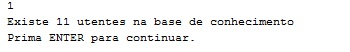
\includegraphics[scale=0.8]{questao1.jpg}
	\caption{Resposta da aplicação à questão quantos utentes estão inseridos no sistema}
\end{figure}

\begin{figure}[<+htb+>]
	\centering
	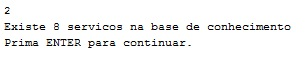
\includegraphics[scale=0.8]{questao2.jpg}
	\caption{Resposta da aplicação à questão qual o nr de serviços registados}
\end{figure}

\begin{figure}[<+htb+>]
	\centering
	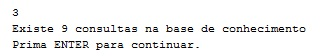
\includegraphics[scale=0.8]{questao3.jpg}
	\caption{Resposta da aplicação à questão qual o nr de serviços registados}
\end{figure}

\begin{figure}[<+ht+>]
	\centering
	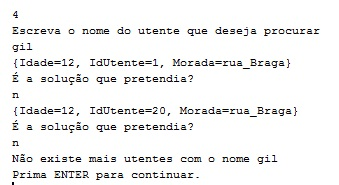
\includegraphics[scale=0.8]{questao4.jpg}
	\caption{Encontrar um utente com um dado nome }
\end{figure}


\begin{figure}[<+ht+>]
	\centering
	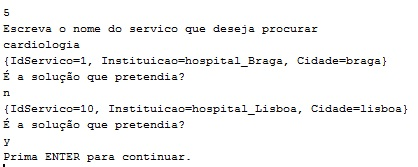
\includegraphics[scale=0.8]{questao5.jpg}
	\caption{Informações sobre determinado serviço}
\end{figure}


\begin{figure}[<+ht+>]
	\centering
	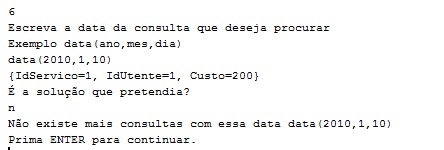
\includegraphics[scale=0.8]{questao6.jpg}
	\caption{Procurar por data de consulta}
\end{figure}

\begin{figure}[<+ht+>]
	\centering
	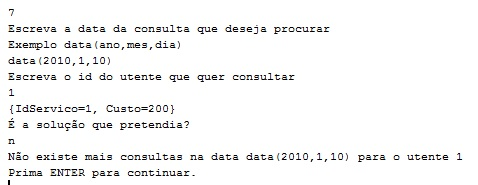
\includegraphics[scale=0.8]{questao7.jpg}
	\caption{Procurar por data de consulta e id de utente}
\end{figure}


\begin{figure}[<+ht+>]
	\centering
	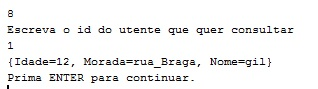
\includegraphics[scale=0.8]{questao8.jpg}
	\caption{Procurar por id de utente}
\end{figure}

\begin{figure}[<+ht+>]
	\centering
	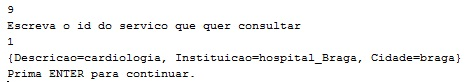
\includegraphics[scale=0.8]{questao9.jpg}
	\caption{Procurar por id de serviço}
\end{figure}

\begin{figure}[<+ht+>]
	\centering
	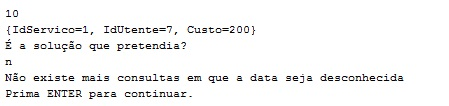
\includegraphics[scale=0.8]{questao10.jpg}
	\caption{Procurar as consultas que não se sabe a data}
\end{figure}

\begin{figure}[<+ht+>]
	\centering
	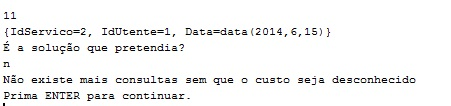
\includegraphics[scale=0.8]{questao11.jpg}
	\caption{Procurar as consultas que não se sabe o custo}
\end{figure}

\begin{figure}[<+ht+>]
	\centering
	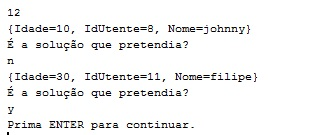
\includegraphics[scale=0.8]{questao12.jpg}
	\caption{Procurar os utentes com morada desconhecida}
\end{figure}



\clearpage

\subsection{Interação com o Sistema em Java}
Foi sugerido que desenvolvessemos uma aplicação Java para tornar o uso do programa mais intuitivo do que o Prolog. Para isso recorremos à biblioteca \textit{Jasper} e criámos um programa com ligação ao \textit{SICStus Prolog}. 

Mostrámos de seguida o menu na figura abaixo com as diversas operações possiveis a realizar: 

\begin{figure}[<+h+>]
	\centering
	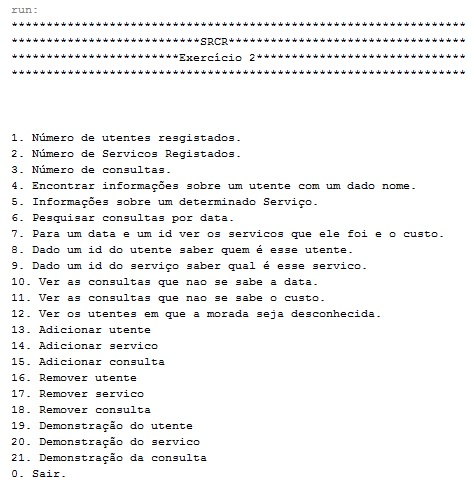
\includegraphics[scale=0.7]{menu.jpg}
	\caption{Menu da aplicação}
\end{figure}



  \begin{minipage}{\linewidth}
  	\centering
  	\begin{minipage}{0.45\linewidth}
  		\begin{figure}[H]
  			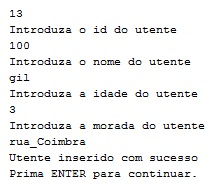
\includegraphics[width=\linewidth]{questao13}
  			\caption{Adicionar Utente}
  		\end{figure}
  	\end{minipage}
  	\hspace{0.05\linewidth}
  	\begin{minipage}{0.45\linewidth}
  		\begin{figure}[H]
  			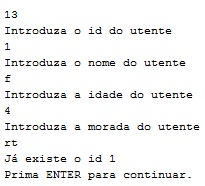
\includegraphics[width=\linewidth]{questao13_falhado}
  			\caption{Exemplo de falha na inserção de um utente já existente}
  		\end{figure}
  	\end{minipage}
  \end{minipage}


  \begin{minipage}{\linewidth}
  	\centering
  	\begin{minipage}{0.45\linewidth}
  		\begin{figure}[H]
  			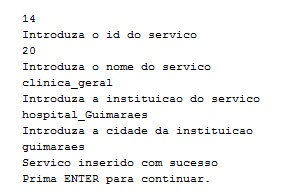
\includegraphics[width=\linewidth]{questao14}
  			\caption{Adicionar Serviço}
  		\end{figure}
  	\end{minipage}
  	\hspace{0.05\linewidth}
  	\begin{minipage}{0.45\linewidth}
  		\begin{figure}[H]
  			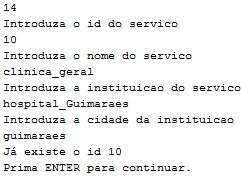
\includegraphics[width=\linewidth]{questao14_falhada}
  			\caption{Exemplo de falha na inserção de um serviço já existente}
  		\end{figure}
  	\end{minipage}
  \end{minipage}

  \begin{minipage}{\linewidth}
  	\centering
  	\begin{minipage}{0.45\linewidth}
  		\begin{figure}[H]
  			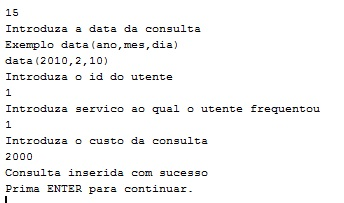
\includegraphics[width=\linewidth]{questao15}
  			\caption{Adicionar Consulta}
  		\end{figure}
  	\end{minipage}
  	\hspace{0.05\linewidth}
  	\begin{minipage}{0.45\linewidth}
  		\begin{figure}[H]
  			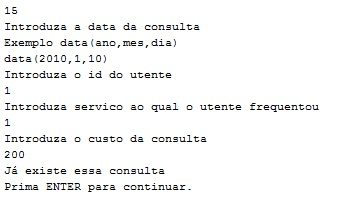
\includegraphics[width=\linewidth]{questao15_falhada}
  			\caption{Exemplo de falha na inserção de uma consulta já existente}
  		\end{figure}
  	\end{minipage}
  \end{minipage}


  \begin{minipage}{\linewidth}
  	\centering
  	\begin{minipage}{0.45\linewidth}
  		\begin{figure}[H]
  			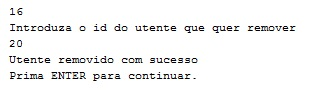
\includegraphics[width=\linewidth]{questao16}
  			\caption{Remover Utente}
  		\end{figure}
  	\end{minipage}
  	\hspace{0.05\linewidth}
  	\begin{minipage}{0.45\linewidth}
  		\begin{figure}[H]
  			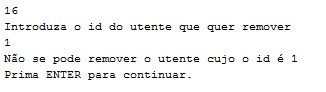
\includegraphics[width=\linewidth]{questao16_falhada}
  			\caption{Exemplo de falha na remoção de um utente}
  		\end{figure}
  	\end{minipage}
  	\hspace{0.05\linewidth}
  		\begin{minipage}{0.45\linewidth}
  			\begin{figure}[H]
  				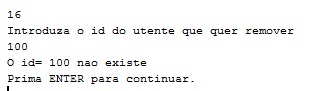
\includegraphics[width=\linewidth]{questao16_idNaoExiste}
  				\caption{Exemplo de falha na remoção de um utente quando este não exite}
  			\end{figure}
  		\end{minipage}
  \end{minipage}
  
  
    \begin{minipage}{\linewidth}
    	\centering
    	\begin{minipage}{0.45\linewidth}
    		\begin{figure}[H]
    			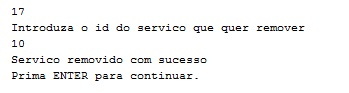
\includegraphics[width=\linewidth]{questao17}
    			\caption{Remover Serviço}
    		\end{figure}
    	\end{minipage}
    	\hspace{0.05\linewidth}
    	\begin{minipage}{0.45\linewidth}
    		\begin{figure}[H]
    			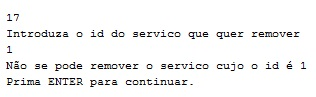
\includegraphics[width=\linewidth]{questao17_falhada}
    			\caption{Exemplo de falha na remoção de um serviço}
    		\end{figure}
    	\end{minipage}
    	\hspace{0.05\linewidth}
    	\begin{minipage}{0.45\linewidth}
    		\begin{figure}[H]
    			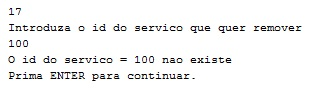
\includegraphics[width=\linewidth]{questao17_idNaoExiste}
    			\caption{Exemplo de falha na remoção de um serviço quando id não existe}
    		\end{figure}
    	\end{minipage}
    \end{minipage}
    
      \begin{minipage}{\linewidth}
      	\centering
      	\begin{minipage}{0.45\linewidth}
      		\begin{figure}[H]
      			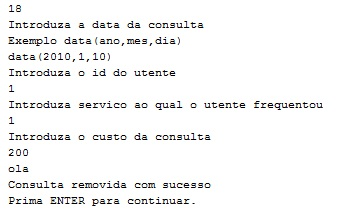
\includegraphics[width=\linewidth]{questao18}
      			\caption{Remover Consulta}
      		\end{figure}
      	\end{minipage}
      	\hspace{0.05\linewidth}
      	\begin{minipage}{0.45\linewidth}
      		\begin{figure}[H]
      			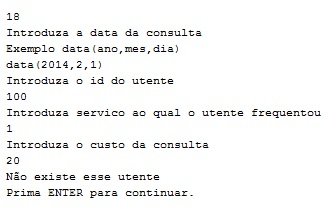
\includegraphics[width=\linewidth]{questao18_UtenteNaoExiste}
      			\caption{Exemplo de falha na remoção de uma consulta quando utente não existe}
      		\end{figure}
      	\end{minipage}
      	\begin{minipage}{0.45\linewidth}
      		\begin{figure}[H]
      			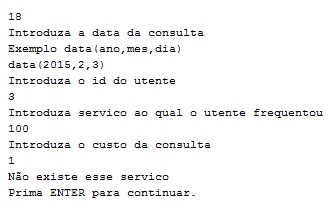
\includegraphics[width=\linewidth]{questao18_ServicoNaoExiste}
      			\caption{Exemplo de falha na remoção de uma consulta quando serviço não existe}
      		\end{figure}
      	\end{minipage}
      	\begin{minipage}{0.45\linewidth}
      	\begin{figure}[H]
      		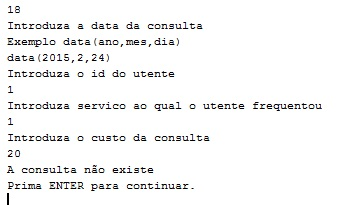
\includegraphics[width=\linewidth]{questao18_ConsultaNaoExiste}
      		\caption{Exemplo de falha na remoção de uma consulta quando consulta não existe}
      	\end{figure}
      \end{minipage}
      \end{minipage}
      
      
  \begin{minipage}{\linewidth}
  	\centering
  	\begin{minipage}{0.45\linewidth}
  		\begin{figure}[H]
  			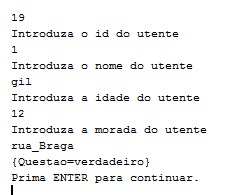
\includegraphics[width=\linewidth]{questao19}
  			\caption{Demo do utente}
  		\end{figure}
  	\end{minipage}
  	\hspace{0.05\linewidth}
  	\begin{minipage}{0.45\linewidth}
  		\begin{figure}[H]
  			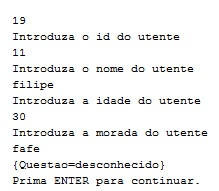
\includegraphics[width=\linewidth]{questao19_ConhecimentoIndeterminado}
  			\caption{Exemplo conhecimento indeterminado}
  		\end{figure}
  	\end{minipage}
  \end{minipage}
      



